%%%%%%%%%%%%%%%%%%%%%%%%%%%%%%%%%%%%%%%%%%%%%%%%%%%%%%%%%%%%%%%%%%%%%%
% LaTeX Example: Project Report
%
% Source: http://www.howtotex.com
%
% Feel free to distribute this example, but please keep the referral
% to howtotex.com
% Date: March 2011 
% 
%%%%%%%%%%%%%%%%%%%%%%%%%%%%%%%%%%%%%%%%%%%%%%%%%%%%%%%%%%%%%%%%%%%%%%
% How to use writeLaTeX: 
%
% You edit the source code here on the left, and the preview on the
% right shows you the result within a few seconds.
%
% Bookmark this page and share the URL with your co-authors. They can
% edit at the same time!
%
% You can upload figures, bibliographies, custom classes and
% styles using the files menu.
%
% If you're new to LaTeX, the wikibook is a great place to start:
% http://en.wikibooks.org/wiki/LaTeX
%
%%%%%%%%%%%%%%%%%%%%%%%%%%%%%%%%%%%%%%%%%%%%%%%%%%%%%%%%%%%%%%%%%%%%%%
% Edit the title below to update the display in My Documents
%\title{Project Report}
%
%%% Preamble
\documentclass[paper=a4, fontsize=11pt]{scrartcl}
\usepackage[T1]{fontenc}
\usepackage{fourier}

\usepackage[english]{babel}                                                         % English language/hyphenation
\usepackage[protrusion=true,expansion=true]{microtype}  
\usepackage{amsmath,amsfonts,amsthm} % Math packages
\usepackage[pdftex]{graphicx}   
\usepackage{url}
\usepackage{physics}
\usepackage{siunitx}
\usepackage{float}

%%% Custom sectioning
\usepackage{sectsty}
\allsectionsfont{\centering \normalfont\scshape}


%%% Custom headers/footers (fancyhdr package)
\usepackage{fancyhdr}
\pagestyle{fancyplain}
\fancyhead{}                                            % No page header
\fancyfoot[L]{}                                         % Empty 
\fancyfoot[C]{}                                         % Empty
\fancyfoot[R]{\thepage}                                 % Pagenumbering
\renewcommand{\headrulewidth}{0pt}          % Remove header underlines
\renewcommand{\footrulewidth}{0pt}              % Remove footer underlines
\setlength{\headheight}{13.6pt}


%%% Equation and float numbering
\numberwithin{equation}{section}        % Equationnumbering: section.eq#
\numberwithin{figure}{section}          % Figurenumbering: section.fig#
\numberwithin{table}{section}               % Tablenumbering: section.tab#


%%% Maketitle metadata
\newcommand{\horrule}[1]{\rule{\linewidth}{#1}}     % Horizontal rule

\title{
        %\vspace{-1in}  
        \usefont{OT1}{bch}{b}{n}
        \normalfont \normalsize \textsc{MIT 18.086 Computational Science and Engineering II} \\ [25pt]
        \horrule{0.5pt} \\[0.4cm]
        \huge Computational Fluid Dynamics with Shocks \\
        \horrule{2pt} \\[0.5cm]
}
\author{
        \normalfont                                 \normalsize
        Matthew Vernacchia\\[-3pt]      \normalsize
        \today
}
\date{}


%%% Begin document
\begin{document}
\maketitle
\section{Abstract}

%%%%%%%%%%%%%%%%%%%%%%%%%%%%%%%%%%%%%%%%%%%%%%%%%%%%%%%%%%%%%%%%%%%%%%%%%%%%%%%
\section{Introduction}
\subsection{Motivation}
Many engineering problems in the military and transportation sectors involve supersonic fluid flow. A significant phenomenon in many supersonic flow problems is the formation of shock waves. Important design problems, such as a helmets to protect against traumatic brain injury from explosions, rocket nozzles for missiles and launch vehicles, or a spacecraft's reentry trajectory, depend on our ability to model and understand shocks.\\
Analytical solutions exist for some simple problems, and these were the primary engineering analysis tools during the 1940s, 50s and 60s. However, these tools restricted designers to simple geometries and a piecewise understanding of the problem. Consider an aircraft designer asked to predict the shock pattern and drag of a fighter jet in supersonic flight. He could solve the shock pattern from a conical nose and from a diamond-section wing or tail, and add these results together to get a rough estimate of the total vehicle's drag. However, the interaction of these shocks where the wing and fuselage meet would be left to guesswork. And a more complicated wing cross section (i.e. a proper airfoil) would not be possible to solve. Therefore, a drag prediction of useful fidelity would require expensive and time consuming wind tunnel tests.\\
Numerical solutions to fluid flow problems (Computational Fluid Dynamics) now enable engineers to analyze more complicated problems. This allows for the design of higher-performance vehicles. Although wind tunnel testing is often still necessary to calibrate or validate CFD results, the use of CFD means that much fewer physical experiments must be performed. This can substantially reduce the cost and time of development.  


\subsection{Governing Equations}
\subsubsection{Navier-Stokes Equations}
Fluid flow (whether subsonic or supersonic) is governed by the Navier Stokes equations. In $n$ dimensions, these equations contain $4 + n$ unknowns at each point in space and time:
\begin{itemize}
    \item Pressure, $p$
    \item Density, $\rho$
    \item Internal energy, $e$
    \item Temperature, $T$
    \item Velocity, $\vec{u}$
\end{itemize}

There are $4 + n$ equations which relate these variables:

\paragraph{Continuity Equation}
The continuity equation enforces the conservation of mass.
\begin{equation}
    \label{eqn:ns_continuity}
    \pdv{\rho}{t} + \nabla \cdot (\rho \vec{u}) = 0
\end{equation}

\paragraph{Momentum Equations}
The momentum equations (one for each spatial dimension) enforce Newton's Laws. They relate the inertia of the fluid to the pressure, viscous, and external forces.
\begin{equation}
    \label{eqn:ns_momentum}
    \pdv{\vec{u}}{t} + \vec{u} \cdot \nabla \vec{u} = - \frac{1}{\rho} \nabla p + \nu \nabla^2 \vec{u} + \frac{1}{3} \nu \nabla (\nabla \cdot \vec{u}) + \vec{F}
\end{equation}
where $\nu$ is the kinematic viscosity (a property of the fluid) and $\vec{F}$ is an external force applied to the fluid per unit mass.

\paragraph{Energy Equation}
The energy equation enforces the conservation of energy. It relates the change in internal energy of the fluid to pressure work, viscous work, and thermal conduction.
\begin{equation}
    \label{eqn:ns_energy}
    \rho(\pdv{e}{t} + \vec{u} \cdot \nabla e) = - p \nabla \vec{u} + \Phi + \nabla \cdot (k \nabla T)
\end{equation}
where $\Phi$ is a viscous term dependent on the velocity second derivatives of velocity and $\nu$, and $k$ is the thermal conductivity (a property of the fluid).

\paragraph{Thermodynamic Relation}
The thermodynamic relation links the internal energy to the temperature and pressure.
\begin{equation}
    \label{eqn:ns_thermo}
    e = e(T, p)
\end{equation}
For a calorically perfect gas,
\begin{equation}
    e = c_v T
\end{equation}
where $c_v$ is the gas's heat capacity at constant volume. Most real gases can be approximated as calorically perfect over small ranges of temperature.

\paragraph{Equation of State}
The equation of state relates the fluid's pressure, density, and temperature.
\begin{equation}
    \label{eqn:ns_state}
    \rho = \rho(p, T)
\end{equation}
A common equation of state is the ideal gas law:
\begin{equation}
    \rho = \frac{p}{R T}
\end{equation}
where $R$ is the specific gas constant (a property of the fluid). For a gas that is also calorically perfect, the ideal gas law can be written as:
\begin{equation}
    \label{eqn:prhoe}
    \rho = \frac{p}{(\gamma - 1) e}
\end{equation}
where $\gamma = c_p / c_v$ is the ratio of specific heats (a property of the fluid).

\subsubsection{Non-Dimensional Parameters}
Two important non-dimensional parameters define flow regimes where the behavior of the Navier-Stokes equations are different.

\paragraph{Mach Number}
The Mach number is the local velocity normalized by the local speed of sound.
\begin{equation}
    M = \frac{|\vec{u}|}{a}
\end{equation}
where $a$ is the local speed of sound (a function of the temperature and fluid properties). Mach numbers less than 1 are subsonic; while Mach numbers greater than one are supersonic.\\
For subsonic flow, the Navier-Stokes equations are classified as elliptic PDEs, and their solutions are smooth. For supersonic flow, the Navier-Stokes PDEs are parabolic: information does not propagate upstream in the flow, and sharp changes in the solution variables (shocks) can exist.

\paragraph{Reynolds Number}
The Reynolds number gives the relative strength of inertia and viscous forces.
\begin{equation}
    Re = \frac{|\vec{u}| L}{\nu}
\end{equation}
Where $L$ is a length scale of the problem, such as the chord of a wing or the diameter of a pipe.\\
If the Reynolds number is high, then viscous forces are small compared to the inertia of the flow, and can be neglected for certain calculations. This leads to an important simplification of the Navier-Stokes equations.

\subsubsection{Euler Equations}
In the context of fluid dynamics, the Euler equations are a simplification of the Navier-Stokes equations, with no viscosity or thermal conductivity ($\nu = k = 0$). They provide a good approximation of certain high Reynolds number problems. The modified momentum and energy equations are written below. The continuity equation (\ref{eqn:ns_continuity}), thermodynamic relation (\ref{eqn:ns_thermo}), and equation of state (\ref{eqn:ns_state}) did not contain viscosity or conductivity terms, and are therefore unchanged.  

\paragraph{Euler Momentum Equation}
\begin{equation}
    \pdv{\vec{u}}{t} + \vec{u} \cdot \nabla \vec{u} = - \frac{1}{\rho} \nabla p + \vec{F}
\end{equation}

\paragraph{Euler Energy Equation}
\begin{equation}
    \rho(\pdv{e}{t} + \vec{u} \cdot \nabla e) = - p \nabla \vec{u}
\end{equation}

The Euler equations are hyperbolic PDEs.

\subsubsection{Euler Equations in Conservative Form}
The Euler equations can be written in a conservative, vectorized, flux-based form. This form is convenient for numerical techniques. I will present the conservative form in 2 dimensions, but it can also be developed in 1 or 3. I assume a 2D Cartesian coordinate system with spatial directions $x$ and $y$. The state of the fluid is represented by the vector $U$ (not to be confused with the velocity vector, $\vec{u}$):
\begin{equation}
    U = 
    \begin{bmatrix}
        \rho \\
        \rho u \\
        \rho v \\
        E
    \end{bmatrix}
\end{equation}
where:
\begin{itemize}
    \item $u$ and $v$ are the velocity components in the $x$ and $y$ directions. $\vec{u} = [u, v]^T$.
    \item $\rho u$ and $\rho v$ are the momentum per unit volume in the the $x$ and $y$ directions. The have units of mass per area-time (\si{\kilo\gram\per\meter\squared\second} in SI).
    \item $E$ is the total energy per unit volume. $E = \rho (e + \frac{1}{2}(u^2 + v^2))$. $E$ has units of energy per volume, which is equal to units of pressure (in SI, \si{\joule\per\meter\cubed} or \si{\pascal}).
\end{itemize}

The state of the fluid is a function of space and time:
\begin{equation}
    U = U(x, y, t)
\end{equation}

Next, define fluxes $F$ and $G$ for the $x$ and $y$ directions:
\begin{equation}
    F = 
        \begin{bmatrix}
            \rho u \\
            \rho u^2 + p \\
            \rho u v \\
            (E + p)u \\
        \end{bmatrix}
\end{equation}
\begin{equation}
    G = 
        \begin{bmatrix}
            \rho v \\
            \rho u v \\
            \rho v^2 + p \\
            (E + p)v \\
        \end{bmatrix}
\end{equation}

The Euler continuity, energy, and momentum equations can be written as:
\begin{equation}
    \pdv{U}{t} + \pdv{F}{x} + \pdv{G}{y} = 0
\end{equation}

Although pressure and temperature are not included in the state vector $U$, they can be uniquely determined from $U$ using the equation of state and thermodynamic relation. In the case of a calorically perfect gas,
\begin{equation}
    p = (\gamma - 1) \left( E - \frac{1}{2} \rho (u^2 + v^2) \right)
\end{equation}

\begin{equation}
    T = \frac{1}{c_v} \left( \frac{E}{\rho} - (u^2 + v^2) \right)
\end{equation}

\subsection{Numerical Techniques}
Many numerical techniques exist for solving the Euler equations. I classify these techniques by 3 choices: the spatial flux scheme, the time update scheme, and the shock capturing technique.\\
In all techniques, the solution is discretized spatially onto a grid or mesh. The state $U$ of each grid node is stored, this set of $U$s represents the state of the system at a point in time. An update function uses this data to calculate the set of $U$s at the next time step.

\subsubsection{Spatial Flux Scheme}
Two major techniques exist for capturing the spatial derivative terms: finite differences and finite volume.

\paragraph{Finite Differences}
In the Finite Difference technique, the fluxes $F$ and $G$ are calculated at each grid point. To find the time derivative of $U$ at grid point $i, j$, one uses the flux values at the neighbor points to estimate the spatial gradients of $F$ and $G$. These gradients can be calculated using a central difference or upwind stencil. Finite difference techniques were the first to be developed, and are simpler to implement.

\begin{figure}[H]
    \centering
    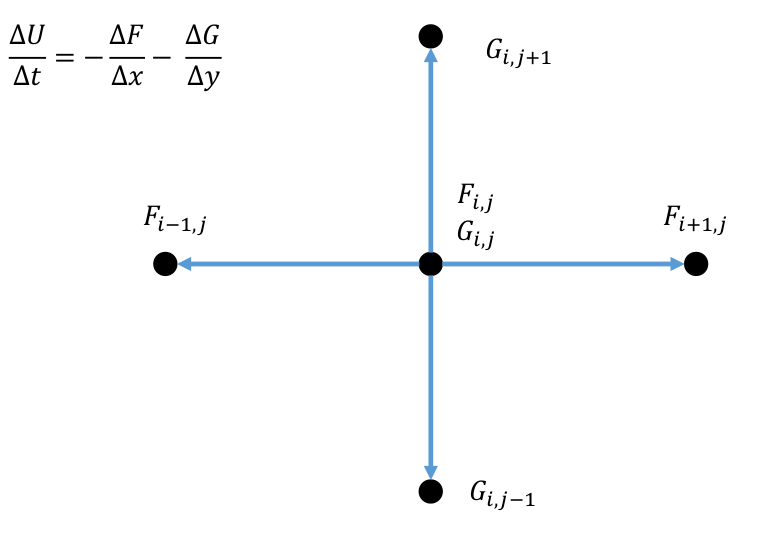
\includegraphics[width = 0.8 \textwidth]{figures/finite_diff.png}
    \caption{Finite Difference scheme.}
    \label{fig:finite_diff}
\end{figure}

\paragraph{Finite Volumes}
In the Finite Volume technique, a boundary $B$ is defined around each grid point, which encloses a finite volume $V$ of space. The fluxes $F$ and $G$ are calculated between grid points, on the sides of $B$. Using the divergence theorem, we write the time rate of change of $U$ within $V$ as surface integral of the fluxes over $B$:
\begin{equation}
    \pdv{}{t} \left( \iint_V U dV \right) = \oint_B (F \hat{x} + G \hat{y}) \cdot \hat{n} dB
\end{equation}

To discretized this equation, we choose $V$ small enough that $U$ can be assumed to have a uniform value within it. Then,

\begin{equation}
    \frac{\Delta U}{\Delta t}_{i,j} = \frac{1}{V} \oint_{B_{i,j}} (F \hat{x} + G \hat{y}) \cdot \hat{n} dB
\end{equation}

The finite volume scheme was developed after finite differences, and is somewhat harder to implement (on a Cartesian grid). However, it is conservative, and is easier to apply to unstructured meshes. Guaranteed conservation and applicability to complicated geometries are valuable for solving engineering problems. Therefore, finite volumes are used in most modern CFD software.

\begin{figure}[H]
    \centering
    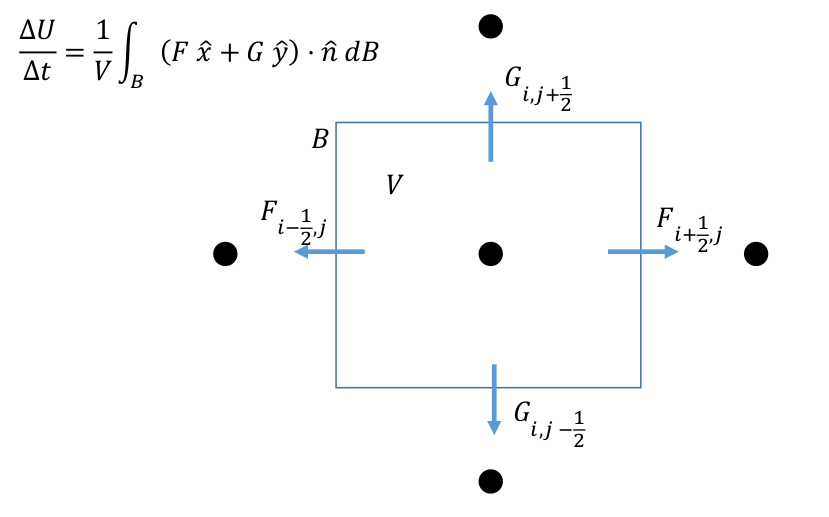
\includegraphics[width = 0.8 \textwidth]{figures/finite_volume.png}
    \caption{Finite Volume scheme.}
    \label{fig:finite_volume}
\end{figure}

\subsubsection{Time Update Scheme}
Several algorithms are used to approximate the integration of $U$ through time. These are broadly divided into explicit and implicit techniques.

\paragraph{Explicit}
Explicit techniques define $U^{n+1}$ as an explicit function of previous time steps $U^{n}, U^{n-1}, ...$. They are usually easier to implement and require less computation per step than implicit techniques. However, their stability is limited to sufficiently small time steps. The Courant-Friedrichs-Lewy (CFL) condition provides an upper bound for the allowable time step:
\begin{equation}
    \Delta t < (\Delta t)_{CFL} = \frac{1}{\frac{|u|}{\Delta x} + \frac{|v|}{\Delta y} + a \sqrt{\frac{1}{\Delta x^2} + \frac{1}{\Delta y^2}}}
\end{equation}

MacCormack is a common explicit method for the Euler and Navier-Stokes equations, but other explicit methods (Runge-Kutta, Lax-Wendroff) have been successfully used as well.

\paragraph{Implicit}
Implicit techniques define an implicit relation between $U^{n+1}$ and $U^n$. To find $U^{n+1}$, a (usually linear) system of equations must be solved. Implicit techniques are more difficult to implement and require more computation at each step (to solve the system of equations). However, their stability is not restricted to small time steps, so (if high resolution in time is not desired) less steps need to be computed, reducing the overall computation requirements.\\

Beam-Warming is a commonly used implicit method.

\subsubsection{Shock Capturing}
Hyperbolic PDEs present a challenge to numerical algorithms. In the case of the Euler equations, solvers tend to exhibit non-physical oscillations near shocks. These oscillations can impart the stability of the algorithm, and reduce the accuracy of the solution. To properly capture flow with shocks, modifications must be made to the algorithm to reduce these oscillations. This is achieved by adding artificial dissipation or limiting the flux.\\

\paragraph{Classical Schemes}
Classical schemes for shock handling use a classical time and gradient scheme (e.g. MacCormack) and add artificial dissipation.

\paragraph{Modern Schemes}
A popular class of modern shock handling schemes are the Total Variation Diminishing (TVD) methods. These have the property the the magnitude of the local extrema of the solution monotonically decrease with time. They handle shocks well, but only provide 1st order spatial accuracy. Newer algorithms include the Monotonic Upstream-centered Schemes for Conservation Laws (MUSCL) and Essentially Non-Oscillatory (ENO) methods.

\begin{figure}[H]
    \centering
    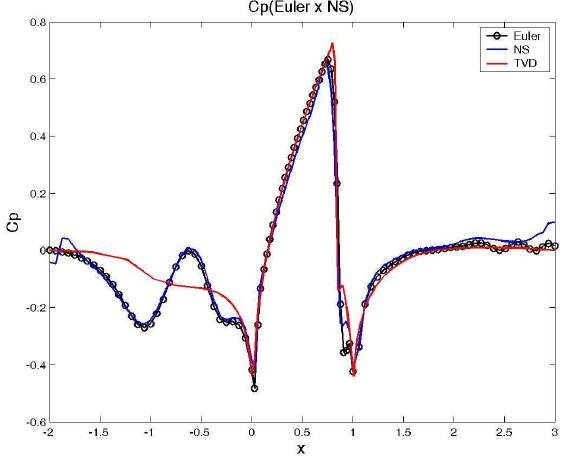
\includegraphics[width = 0.8 \textwidth]{figures/lobao_mc_tvd.png}
    \caption{A comparison of shock capturing schemes. This figure shows the coefficient of pressure along the surface of a wall. The wall has a small parabolic bump the protrudes into the flow from $x = 0$ to $x = 1$. The inlet flow is subsonic ($M= 0.85$) but the fluid accelerates to sonic speed over the bump, and a shock exists at the rear of the bump. A MacCormack solver with artificial dissipation (black curve) gives non-physical pressure oscillations upstream of the bump. A TVD solver (red curve) does not. Figure reprinted from D. Lobao 2010.}
    \label{fig:lobao_mc_tvd}
\end{figure}


%%%%%%%%%%%%%%%%%%%%%%%%%%%%%%%%%%%%%%%%%%%%%%%%%%%%%%%%%%%%%%%%%%%%%%%%%%%%%%%
\section{Implementation}
\subsection{Computation Platform}
I implemented my solver in the Julia programming language (v 0.4.2). I performed my computations on a laptop computer with 6 GB RAM and an Intel i5-2410M CPU (2 cores at $\SI{2.3}{\giga\hertz}$) running 64 bit Ubuntu 14.04.

\subsection{Solver}
\subsubsection{Time Update: MacCormack Scheme}

\subsubsection{Shock Capturing: Artificial Dissipation}

\subsubsection{Curvilinear Coordinates}

\subsubsection{Boundary Conditions}


%%%%%%%%%%%%%%%%%%%%%%%%%%%%%%%%%%%%%%%%%%%%%%%%%%%%%%%%%%%%%%%%%%%%%%%%%%%%%%%
\section{Results}
\subsection{Shock Tube}

\subsection{Mach $1.5$ Ramp}

%%%%%%%%%%%%%%%%%%%%%%%%%%%%%%%%%%%%%%%%%%%%%%%%%%%%%%%%%%%%%%%%%%%%%%%%%%%%%%%
\section{Conclusion}

\end{document}